% \begin{document}
\section{Hungarian Method}
\subsection{Duality and Complementarity Slackness of Min-Cost Perfect Matching}

Let $G=(A\cup B,E)$ be a bipartite weighted graph with edge-costs $c:E\to\mathbb{R}$. We wish to
find a perfect matching $M$ of minimum cost $\sum_{e\in M}c(e)$.

To write down the linear program for this problem, we have a variable $x_e$ for every edge $e$,
with the intended meaning that $x_e$ takes value $1$ if $e$ is in the matching and $0$ otherwise.
In a perfect matching, every vertex is adjacent to exactly one edge of the matching. This leads to
the following linear program:
\begin{center}
\begin{tabular}{ll}
  Minimize    & $\displaystyle\sum_{e\in E}c(e)x_e$\\[8pt]
  Subject to: & $\displaystyle\sum_{b\in B:(a,b)\in E}x_{ab}=1\quad\forall a\in A,$\\[8pt]
              & $\displaystyle\sum_{a\in A:(a,b)\in E}x_{ab}=1\quad\forall b\in B,$\\[8pt]
              & $x_e\ge 0\quad\forall e\in E.$
\end{tabular}
\end{center}
In a previous lecture, we saw that any extreme point of the above linear program is integral.
Hence, we could solve the min-cost perfect matching problem by simply solving the above linear
program, finding an extreme-point solution. However, this may be unnecessarily inefficient.
Instead, we will see how to use LP duality to, basically, reduce this (weighted) problem to that
of finding a perfect matching in an unweighted graph. (A problem that we already saw how to solve
using augmenting paths.)

\paragraph{Obtaining the dual.} To take the dual of the above program, let us first write it in
the same form as last lecture, i.e.\ a minimization problem with $\ge$ and nonnegativity
constraints. We can do this by replacing each equality by two inequalities. This gives us the
following equivalent linear program:
\begin{center}
\begin{tabular}{ll}
  Minimize    & $\displaystyle\sum_{e\in E}c(e)x_e$\\[8pt]
  Subject to: & $\displaystyle\sum_{b\in B:(a,b)\in E}x_{ab}\ge 1\quad\forall a\in A,$\\[8pt]
              & $\displaystyle-\sum_{b\in B:(a,b)\in E}x_{ab}\ge -1\quad\forall a\in A,$\\[8pt]
              & $\displaystyle\sum_{a\in A:(a,b)\in E}x_{ab}\ge 1\quad\forall b\in B,$\\[8pt]
              & $\displaystyle-\sum_{a\in A:(a,b)\in E}x_{ab}\ge -1\quad\forall b\in B,$\\[8pt]
              & $x_e\ge 0\quad\forall e\in E.$
\end{tabular}
\end{center}
For each $a\in A$, we then associate a variable $u_a^+$ to the first constraint for $a$
($\sum_{b\in B:(a,b)\in E}x_{ab}\ge 1$) and $u_a^-$ to the second constraint for $a$
($-\sum_{b\in B:(a,b)\in E}x_{ab}\ge -1$). Similarly, we have variables $v_b^+$ and $v_b^-$ for
each $b\in B$. These variables take the same role as the $y$-variables: the dual has
a variable for each constraint in the primal. We now have that the dual equals
\begin{center}
\begin{tabular}{ll}
  Maximize    & $\displaystyle\sum_{a\in A}(u_a^+-u_a^-)+\sum_{b\in B}(v_b^+-v_b^-)$\\[8pt]
  Subject to: & $(u_a^+-u_a^-)+(v_b^+-v_b^-)\le c(e)\quad\forall e=(a,b)\in E,$\\[4pt]
              & $u_a^+,u_a^-,v_b^+,v_b^-\ge 0\quad\forall a\in A,\ b\in B.$
\end{tabular}
\end{center}

\paragraph{Complementarity Slackness.} Complementarity slackness tells us that if
$x,(u^+,u^-,v^+,v^-)$ are feasible, then they are both optimal if and only if the following holds:
\begin{align*}
  x_e>0 &\Rightarrow (u_a^+-u_a^-)+(v_b^+-v_b^-)=c(e) && \forall e=(a,b)\in E,\\
  u_a^+>0 &\Rightarrow \sum_{b\in B:(a,b)\in E}x_{ab}=1 && \forall a\in A,\\
  u_a^->0 &\Rightarrow -\sum_{b\in B:(a,b)\in E}x_{ab}=-1 && \forall a\in A,\\
  v_b^+>0 &\Rightarrow \sum_{a\in A:(a,b)\in E}x_{ab}=1 && \forall b\in B,\\
  v_b^->0 &\Rightarrow -\sum_{a\in A:(a,b)\in E}x_{ab}=-1 && \forall b\in B.
\end{align*}
We have thus obtained the dual and the complementarity slackness conditions in an ``automatic''
way.

\paragraph{Simplifying the notation.} Before continuing, we would like to make an observation that
will simplify our description and notation. Namely, in the dual that we obtained, the variables
$u_a^+$ and $u_a^-$ always appear only as part of the expression $(u_a^+-u_a^-)$. Although we have
$u_a^+,u_a^-\ge 0$, this expression can take any value (positive and negative). We can thus for
every $a\in A$ replace $(u_a^+-u_a^-)$ by a new variable $u_a\in\mathbb{R}$ whose value is not
constrained to be nonnegative (it can take both positive and negative values). We do the same for
each $b\in B$ and replace $(v_b^+-v_b^-)$ by $v_b$.\footnote{Note that our new LP is in fact
equivalent to the old one. Given a feasible solution to the old LP, we can obtain a feasible
solution to the new LP by setting the values for the new variables as $u_a:=u_a^+-u_a^-$ (and
similarly for $v$). Since we do the same in the objective function, the objective value remains
unchanged. We can also go back and obtain a solution of the old LP from a solution of the new LP
as follows: if $u_a\ge 0$, set $u_a^+=u_a$ and $u_a^-=0$; otherwise set $u_a^+=0$ and
$u_a^-=-u_a$ (and similarly for $v$).

\par\smallskip
Also note that the new LP is what we would have obtained if we had multiplied each equality
constraint $\sum_{b\in B:(a,b)\in E}x_{ab}=1$ by an unconstrained dual variable $u_a\in\mathbb{R}$,
rather than rewriting this equality constraint as two inequality constraints and then multiplying
each by a nonnegative dual variable ($u_a^+$ or $u_a^-$). (And similarly for $v$.)} We can thus
write the primal and the dual as follows:
\begin{center}
\begin{tabular}{ll}
  Minimize    & $\displaystyle\sum_{e\in E}c(e)x_e$\\[8pt]
  Subject to: & $\displaystyle\sum_{b\in B:(a,b)\in E}x_{ab}=1\quad\forall a\in A,$\\[8pt]
              & $\displaystyle\sum_{a\in A:(a,b)\in E}x_{ab}=1\quad\forall b\in B,$\\[8pt]
              & $x_e\ge 0\quad\forall e\in E.$
\end{tabular}
\end{center}
and
\begin{center}
\begin{tabular}{ll}
  Maximize    & $\displaystyle\sum_{a\in A}u_a+\sum_{b\in B}v_b$\\[8pt]
  Subject to: & $u_a+v_b\le c(e)\quad\forall e=(a,b)\in E.$
\end{tabular}
\end{center}
With this simplified notation, complementarity slackness gives us that if $x,(u,v)$ are feasible,
then they are both optimal if and only if the following holds:
\begin{align*}
  x_e>0 &\Rightarrow u_a+v_b=c(e) && \forall e=(a,b)\in E,\\
  u_a\neq 0 &\Rightarrow \sum_{b\in B:(a,b)\in E}x_{ab}=1 && \forall a\in A,\\
  v_b\neq 0 &\Rightarrow \sum_{a\in A:(a,b)\in E}x_{ab}=1 && \forall b\in B.
\end{align*}
As a final simplification, observe that the last two conditions always hold since they follow
immediately from the fact that $x$ is primal-feasible (this is because in this LP we have
equalities instead of inequalities). We can thus summarize the above with the following:
\label{lem:cs}
\mlenma{}{
A perfect matching $M$ is of minimum cost iff there is a feasible dual solution $u,v$ such that
$u_a+v_b=c(e)$ for every $e=(a,b)\in M$.
}

\subsection{The Hungarian Algorithm}

We start with some intuition before we give the formal description of the algorithm.

\subsubsection*{Intuition}

Consider the following instance of the min-cost perfect matching problem:

\begin{center}
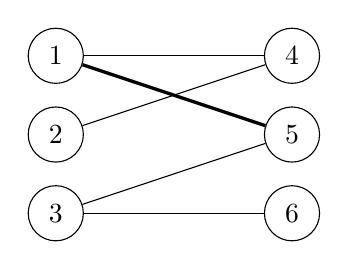
\begin{tikzpicture}[every node/.style={circle,draw,minimum size=7mm,inner sep=0pt}]
  \node (1) at (0,2) {1};
  \node (2) at (0,1) {2};
  \node (3) at (0,0) {3};
  \node (4) at (3,2) {4};
  \node (5) at (3,1) {5};
  \node (6) at (3,0) {6};
  \draw (1) -- (4);
  \draw (2) -- (4);
  \draw (3) -- (5);
  \draw (3) -- (6);
  \draw[very thick] (1) -- (5);
\end{tikzpicture}
\end{center}

The thin edges have cost $1$, whereas the thick edge has cost $2$. The Hungarian algorithm will
use Lemma~\ref{lem:cs} in the following way: we will maintain a dual solution $u,v$ that is
feasible at all times. Then, for a fixed dual solution, the lemma tells us that our perfect
matching is only allowed to contain edges that are \emph{tight}, i.e., edges $e=(a,b)$ for which
$u_a+v_b=c(e)$. This reduces our problem to finding any perfect matching in the subgraph
consisting only of tight edges, i.e., in the graph $(V,E_0)$ where
$E_0=\{e=(a,b)\in E: u_a+v_b=c(e)\}$. Intuitively, we have thus reduced our weighted problem to
an unweighted one!

Let us return to our example. We initialize our procedure with the trivial dual solution
\[
  v_b=0,\qquad u_a=\min_{b\in B}c_{ab}.
\]
(We could have also started from $u=v=0$.) So in the example, $v_4=v_5=v_6=0$ and
$u_1=u_2=u_3=1$. The set $E_0$ of tight edges is thus:

\begin{center}
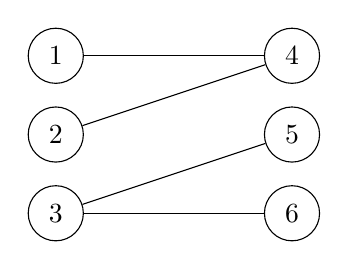
\begin{tikzpicture}[every node/.style={circle,draw,minimum size=7mm,inner sep=0pt}]
  \node (1) at (0,2) {1};
  \node (2) at (0,1) {2};
  \node (3) at (0,0) {3};
  \node (4) at (3,2) {4};
  \node (5) at (3,1) {5};
  \node (6) at (3,0) {6};
  \draw (1) -- (4);
  \draw (2) -- (4);
  \draw (3) -- (5);
  \draw (3) -- (6);
\end{tikzpicture}
\end{center}

We then try to find a perfect matching in this graph using e.g.\ the augmenting path algorithm we
saw in Lecture 3. However, the considered graph has no perfect matching! This is because we
started with a poor lower bound (dual solution). So we will use the fact that there is no perfect
matching to improve our dual solution. We make use of Hall's condition:
\label{thm:hall}
\thm{Hall's Theorem}{
An $n$-by-$n$ bipartite graph $G=(A\cup B,E_0)$ has a perfect matching if and only if
$|S|\le|N(S)|$ for all $S\subseteq A$, where:
\[
N(S)=\{b\in B:\text{there is an } a\in S \text{ such that } (a,b)\in E_0\}
\]
}

\pf{}{
  Lasciata a DarioIlDistruttore
}

Here $N(S)$ denotes the neighborhood of the vertices in $S$.

In the above example, we have $S=\{1,2\}$ and $N(S)=\{4\}$, which violates Hall's condition (and
thus there is no perfect matching). We now use the set $S$ to improve our dual lower bound.

We gradually increase $u_a$ for every $a\in S$ and at the same time decrease $v_b$ for
$b\in N(S)$ at the same rate. Let us see what happens to all edges in $E_0$. Notice that the tight
edges between $S$ and $N(S)$ will remain tight. Similarly, the tight edges between $A\setminus S$
and $B\setminus N(S)$ will remain tight. Any tight edges between $A\setminus S$ and $N(S)$ will
stop being tight. Finally, by definition, there are no edges from $S$ to $B\setminus N(S)$
initially. We continue to gradually change the dual solution until some such edge becomes tight.

In the above example, this will result in updating $u_1=u_2=2$ and $v_4=-1$. We have thus
increased two variables by one unit and decreased one variable by one unit. In total, the dual
lower bound was thus increased by one. The set $E_0$ of tight edges with respect to the new dual
solution is now

\begin{center}
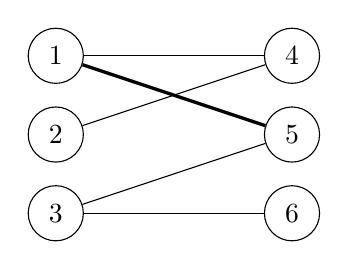
\begin{tikzpicture}[every node/.style={circle,draw,minimum size=7mm,inner sep=0pt}]
  \node (1) at (0,2) {1};
  \node (2) at (0,1) {2};
  \node (3) at (0,0) {3};
  \node (4) at (3,2) {4};
  \node (5) at (3,1) {5};
  \node (6) at (3,0) {6};
  \draw (1) -- (4);
  \draw (2) -- (4);
  \draw (3) -- (5);
  \draw (3) -- (6);
  \draw[very thick] (1) -- (5);
\end{tikzpicture}
\end{center}

Our (augmenting-path) algorithm will now find a perfect matching in this graph, which is optimal
by Lemma~\ref{lem:cs}.\\

In summary, our algorithm always maintains a dual feasible solution. We then solve the unweighted
perfect matching problem on the edges allowed by Lemma~\ref{lem:cs}. In the case of failure,
we update the dual lower bound to a strictly better lower bound and repeat.

\subsubsection*{Formal description}

\textbf{Idea:} Maintain a feasible dual solution $(u,v)$. Try to construct a feasible primal
solution that satisfies complementarity slackness (Lemma~\ref{lem:cs}) and is thus optimal.

\medskip
\noindent\textbf{Algorithm:}
\begin{itemize}
  \item \textbf{Initialization:} $v_b=0,\ u_a=\min_{b\in B}c_{ab}$.
  \item \textbf{Iterative step:}
  \begin{itemize}
    \item consider $G_0=(A\cup B,E_0)$ where $E_0=\{e=(a,b)\in E: u_a+v_b=c(e)\}$ ($E_0$ is the
      set of all tight edges);
    \item find a maximum-cardinality matching in $G_0$:
    \begin{itemize}
      \item if it is a perfect matching, then we are done (this is a primal feasible solution and
        it satisfies complementarity slackness, because we consider only the edges in $E_0$ and
        all of them satisfy slackness by construction),
      \item otherwise the algorithm finds a set $S\subseteq A$ s.t.\ $|S|>|N(S)|$ (which is
        guaranteed to exist by Hall's theorem)
    \end{itemize}
    \item we can choose a small $\varepsilon>0$ and improve the dual solution:
    \[
      u'_a=\begin{cases}u_a+\varepsilon & \text{if } a\in S,\\ u_a & \text{if } a\notin S,\end{cases}
      \qquad
      v'_b=\begin{cases}v_b-\varepsilon & \text{if } b\in N(S),\\ v_b & \text{if } b\notin N(S),\end{cases}
    \]
    which remains dual feasible because:
    \begin{itemize}
      \item edges in $S\times N(S)$ are unchanged ($+\varepsilon-\varepsilon$),
      \item edges in $(A\setminus S)\times(B\setminus N(S))$ are unchanged,
      \item edges in $(A\setminus S)\times N(S)$ are decreased by $\varepsilon$,
      \item edges in $S\times(B\setminus N(S))$ are increased by $\varepsilon$ but they were not
        tight (they were not in $E_0$),
    \end{itemize}
    \item the dual value increases by $(|S|-|N(S)|)\varepsilon$;
    \item to make as much progress as possible (and to get a new tight edge), we should choose
      $\varepsilon$ as large as possible for which the dual remains feasible, that is
      \[
        \varepsilon=\min_{e=(a,b)\in S\times(B\setminus N(S))}c(e)-u_a-v_b>0.
      \]
  \end{itemize}
\end{itemize}

The above algorithm can be implemented to run in time $O(n^3)$. (This is quite non-trivial to see.
It is somewhat easier to implement in $O(n^4)$.)

\subsection*{An alternative proof that the bipartite perfect matching polytope is integral}

We have shown that for any cost function $c$ we can obtain a minimum-cost perfect matching and it
will be integral. By carefully choosing the cost function, one can make any extreme point of the
polytope to be the unique optimum solution to the minimum-cost perfect matching problem. This
shows that all extreme points are integral, i.e., it is an integral polytope. See Figure~\ref{fig:poly}
for an example.

\begin{figure}[h]
\centering
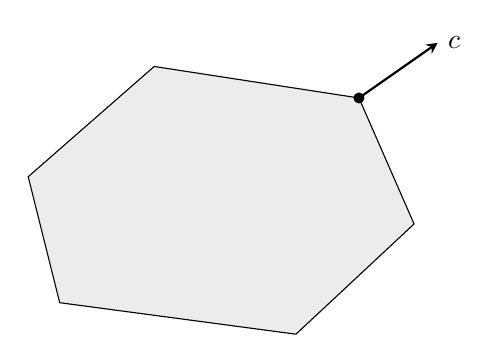
\begin{tikzpicture}[>=stealth]
  \draw[fill=gray!15] (0,0) -- (3,-0.4) -- (4.5,1) -- (3.8,2.6) -- (1.2,3) -- (-0.4,1.6) -- cycle;
  \fill (3.8,2.6) circle (2pt);
  \draw[->,thick] (3.8,2.6) -- (4.8,3.3) node[right] {$c$};
\end{tikzpicture}
\caption{Example of a perfect matching polytope and a cost function vector $c$ for the highlighted
vertex.}
\label{fig:poly}
\end{figure}
% \end{document}
